\documentclass[12pt, a4paper]{article}

% #####################################################################################################################
%
% Title:           Documentation for the script plotspectrum
%
% Author:          Benjamin Bulheller
%
% Website:         www.bulheller.com
%
% Mail address:    webmaster.-at-.bulheller.com
%
% Version:         $Revision$, $Date$
%
% Licence:         This program is free software: you can redistribute it and/or modify
%                  it under the terms of the GNU General Public License as published by
%                  the Free Software Foundation, either version 3 of the License, or
%                  (at your option) any later version.
%
%                  This program is distributed in the hope that it will be useful,
%                  but WITHOUT ANY WARRANTY; without even the implied warranty of
%                  MERCHANTABILITY or FITNESS FOR A PARTICULAR PURPOSE.  See the
%                  GNU General Public License for more details.
%
%                  You should have received a copy of the GNU General Public License
%                  along with this program.  If not, see http://www.gnu.org/licenses/.
%
% #####################################################################################################################

\usepackage{graphicx}
\usepackage[super, square, sort&compress]{natbib}
\usepackage[margin=2.5cm]{geometry}

\setlength{\parskip}{1em}
\setlength{\parindent}{0em}

\setcounter{secnumdepth}{-2}

\clubpenalty=1000
\widowpenalty=1000

\title{plotspectrum}
\author{Benjamin Bulheller\\ \small www.bulheller.com\\ \small webmaster.-at-.bulheller.com}

\begin{document}
\maketitle

{
\linespread{1.0}\normalsize
\setlength{\parskip}{0.4em}
\tableofcontents
}

%%%%%%%%%%%%%%%%%%%%%%%%%%%%%%%%%%%%%%%%%%%%%%%%%%%%%%%%%%%%%%%%%%%%%%%%%%%%%%%%%%%%%%%%%%%%%%%%%%%%

\section*{Licence}

\noindent
Copyright \copyright\ 2009 Benjamin Bulheller, www.bulheller.com \\[1ex]
This program is free software: you can redistribute it and/or modify it under the terms of the GNU General Public License as published by the Free Software Foundation, either version 2 of the License, or (at your option) any later version. \\[1ex]
This program is distributed in the hope that it will be useful, but WITHOUT ANY WARRANTY; without even the implied warranty of MERCHANTABILITY or FITNESS FOR A PARTICULAR PURPOSE.  See the GNU General Public License for more details. \\[1ex]
You should have received a copy of the GNU General Public License along with this program.  If not, see http://www.gnu.org/licenses/. \\[1ex]

\newpage

%%%%%%%%%%%%%%%%%%%%%%%%%%%%%%%%%%%%%%%%%%%%%%%%%%%%%%%%%%%%%%%%%%%%%%%%%%%%%%%%%%%%%%%%%%%%%%%%%%%%

\section{Introduction}

gnuplot\cite{gnuplot} is an extremely powerful interactive data and function plotting utility. Apart from being cross-platform (available for virtually every operating system out there) and command-line driven it is scriptable and supports all conceivable types of graphs and functions.

\verb'plotspectrum' was started to quickly plot circular and linear dichroism spectra (CD, LD) from $xy$-data during a computational chemistry PhD project. One additional option here, another one there, ... and it basically grew into a fully-fledged gnuplot front-end which can either be used to create the rough gnuplot command file in order to edit and perfect afterwards and also comes in handy in scripts when dozens or hundreds of plots need to be produced. It offers lots of command line options to produce quite fine-tunable 2D and 3D plots from one or multiple $xy$-data files using just one (admittedly quite long) command line. It has to be mentioned that I have never used another gnuplot front-end before and therefore I am unsure whether \verb'plotspectrum' actually deserves this ``title''. This also means that I do not know about its shortcomings, which may be satisfied by ``real'' front-ends. I am \emph{more} than happy to look into adding features requested by users and of course I am happy about feedback in general (webmaster.-at-.bulheller.com)!

The powers of gnuplot clearly go beyond the possibility of using it via the command line only and it is \emph{strongly} recommended to become familiar with the syntax and commands of gnuplot command files to harness these possibilities. \verb'plotspectrum', apart from conveniently plotting spectra from the command line also, produces the gnuplot command file which makes it possible to further improve the plots and to learn the syntax and commands this way.

When the number of command line options was found to be headed towards 50 and the usage was spread over two screens this manual was started. Each section generally starts with the usage output of the script, that is all parameters needed for this section. Every parameter is then explained in detail.

The general usage of \verb'plotspectrum' is

\begin{verbatim}
plotspectrum file1 [file2] [...] [options]
\end{verbatim}

where \verb'fileX' contains the $xy$-data in tab- or spaces-separated columns like this:

\begin{verbatim}
#       x-values         y-values
      441.600000         0.038725
      441.700000         0.037447
      441.800000         0.036205
\end{verbatim}

Comment lines are possible and have to start with a hash-symbol (\verb'#'). One or multiple files can be given and are all plotted in the same plot using different line styles by default. \verb'[options]' represents one or more of the various command line parameters which will be discussed in detail.



%%%%%%%%%%%%%%%%%%%%%%%%%%%%%%%%%%%%%%%%%%%%%%%%%%%%%%%%%%%%%%%%%%%%%%%%%%%%%%%%%%%%%%%%%%%%%%%%%%%%


\section{Installation}

The script was written in Perl which is an interpreted language and therefore does not require a compilation. Linux and Mac OS have Perl automatically installed, Windows users need to install ActivePerl\cite{ActivePerl} and have to do some adjustments (e.g. the path to the Perl executable in the first line of the script). However, the script has not been tested under Windows and may not run especially due to possible differences when running gnuplot via the command line.

Under Linux and Mac OS the file needs to be made executable:
\begin{verbatim}
chmod +x plotspectrum
\end{verbatim}

It should then be copied into a folder which is included in the \verb'PATH' so that it can be executed from anywhere in the system without always typing the absolute location of the script. A common folder for user scripts is \verb'~/bin' for example.

The script requires several Perl libraries from which it uses routines. In particular these are
\begin{itemize}
\item \verb'GetParameters.pm' to parse the command line parameters
\item \verb'ReadSpectrum.pm' to read in xy data
\item \verb'GetBaseName.pm' to split a filename into base name and extension
\item \verb'DebugPrint.pm' which comes in handy during debugging
\end{itemize}

These libraries need to be either in one of Perl's library directories, \verb'~/bin/perllib' or in the directory of \texttt{plotspectrum} itself.

If the script is found and no problems occur with the required Perl libraries, issuing the command \verb'plotspectrum' should display the usage information.

The latter three libraries are straightforward to use, without many bells and whistles, and if you would like to use them yourself there are instructions in their headers. The first one, \verb'GetParameters.pm', is a relatively sophisticated command line parameter parser similar to \verb'GetOpt.pm' or \verb'GetOpt-EvaP.pm'. It comes with its own manual offered at www.bulheller.com.


%%%%%%%%%%%%%%%%%%%%%%%%%%%%%%%%%%%%%%%%%%%%%%%%%%%%%%%%%%%%%%%%%%%%%%%%%%%%%%%%%%%%%%%%%%%%%%%%%%%%

\newpage

\section{The Quick'n'Dirty-Section for the Impatient}

I am well aware of the general laziness of users when it comes to reading manuals (being a user myself, that is) and my own pathological wordiness when it comes to write stuff. Therefore, although I really recommend reading or at least skimming through the other sections, I shall provide you with some quick examples that should help to get you started. The command line will start short and will be extended and tuned while adding more bells and whistles. That is, all given lines are actually one command, the previously given ones are abbreviated by \verb'[...]'.

Let's say you want to plot three files with nice keys for each in the legend and a title for the plot:

\begin{verbatim}
plotspectrum spectrum01.cd spectrum02.cd spectrum03.cd \
             -t "CD Spectra of Proteins" \
             -k "helical proteins" "beta sheet proteins" "PPII proteins"
\end{verbatim}

(A trailing backslash tells bash that the command continues on the next line.) This command will plot the three files with the three keys and title (Fig.~\ref{Fig:Plots}, top left). Since the script was developed for plotting CD spectra and recognising the \verb'.cd' extension the script automatically sets the proper axes labels. For the sake of completeness, you may want to change both range and labels:

\begin{verbatim}
    [...] -x 180 250 -y -18000 24000 -xlabel Wavelength -ylabel Intensity
\end{verbatim}

See Fig~\ref{Fig:Plots}, top middle. You could ask for solid lines only (\verb'-solid') or not using colour (\verb'-nocolour'). However, let's make it a little more sophisticated by defining an individual style for each of the files. Similar to giving keys via \verb'-k', one can assign the line type, point type and line width for each given file one after another:

\begin{verbatim}
   [...] -lt 3 6 9   -lc blue red green   -lw 4 8 12 \
\end{verbatim}

Mind that the abbreviations for the options are the same used by gnuplot when defining the line styles. The result is shown in Fig.~\ref{Fig:Plots}, top right. A problem becomes apparent there, it is actually a shortcoming of gnuplot. The length of dashes cannot be defined and the line styles look a bit akward. \verb'plotspectrum' is able to change that directly in the postscript file after creating it, using the respective postscript commands as options. It's a little trying until one finds pleasing values, these lead the result shown in Fig.~\ref{Fig:Plots}, bottom left:

\begin{verbatim}
   [...]  -d 3    -dl1 25 \
\end{verbatim}

For finishing touches you may want to move the legend out of the plot, increase the length of the line samples and -- while you're at it -- increase the line spacing of the legend. All commands referring to the key are the actual gnuplot command prepended with a \verb'k' (Fig.~\ref{Fig:Plots}, bottom right):

\begin{verbatim}
   [...]  -koutside   -ksamplen 4   -kspacing 5
\end{verbatim}

At last, you may want to define the name of the output file (otherwise \verb'plotspectrum' would use the first file with \verb'.ps' extension) and request to keep the actual gnuplot command file in order to tweak it yourself afterwards. If you want to create a PDF from the PS, you can tell the script to do so right away:

\begin{verbatim}
   [...]  -o GreatPlot.ps   -cmd   -pdf
\end{verbatim}



\begin{figure}[h!]
\centering
\includegraphics[width=4cm, angle=-90]{plot01.ps}\hspace{-2em}
\includegraphics[width=4cm, angle=-90]{plot02.ps}\hspace{-2em}
\includegraphics[width=4cm, angle=-90]{plot03.ps}

\includegraphics[width=3.7cm, angle=-90]{plot04.ps}
\includegraphics[width=4cm, angle=-90]{plot05.ps}
\label{Fig:Plots}
\end{figure}


For the sake of completeness, the whole command line which creates the last version of the plot is

\begin{verbatim}
plotspectrum 1rhd.exp.cd 4gcr.exp.cd 2cga.exp.cd -t "CD Spectra of Proteins" \
             -k "helical proteins" "beta sheet proteins" "PPII proteins" \
             -x 180 250 -y -18000 24000 -xlabel Wavelength -ylabel Intensity \
             -lt 3 6 9 -lc blue red green -lw 4 8 12 \
             -d 3 -dl1 25 \
             -koutside -ksamplen 4 -kspacing 5 \
             -o plot05.ps -pdf -cmd
\end{verbatim}

This is of course a \emph{long} command, however, the intention when creating the script in the first place was to make gnuplot scriptable (and it had been used for that purpose to create several hundred plots with one script execution). If one knows the command line switches \verb'plotspectrum' can speed up the creation of the gnuplot command file a great deal.


%%%%%%%%%%%%%%%%%%%%%%%%%%%%%%%%%%%%%%%%%%%%%%%%%%%%%%%%%%%%%%%%%%%%%%%%%%%%%%%%%%%%%%%%%%%%%%%%%%%%


\section{Input, Output, Command and Configuration Files}

\begin{verbatim}
plotspectrum file1 [file2] [...] [options]

    file1       the extension .cd or .ld is added if omitted 
 
    -cmd        keep the gnuplot command file for later changes 
    -cfg        create a .cfg file with the used command line
    -pdf        create a pdf from the postscript 
    -gif        create a GIF file instead of postscript (automatically,
                if .gif extension is given with -o)
    -res        defines the gif resolution xres yres (default 1024,768) 
 
    -o          define a file name of the output file 
    -p          preview mode: open gnuplot instead of writing to a file 
    -s          define the size of the plot (default is $Options->{s}) 
\end{verbatim}

One or more input files (\texttt{file1}, \texttt{file2}, etc.) can be given and will all be plotted in the same plot with different line styles. The files need to contain $xy$ data, that is two columns with numbers separated by tabs or spaces. Comment lines are possible starting with a hash symbol (\verb'#'). Every file is checked for existence and if not found the extensions \verb'.cd' and \verb'.ld' are tested. That is, these extensions may be omitted on the command line.

Via \verb'-o outfile' an output file can be defined (the extension \verb'.ps' is automatically added if it is omitted). If \verb'-o' is not given then the base name of the first input file is used (output to a postscript file is default). To output to a GIF file, the parameter \verb'-gif' can be given. If an output file with \verb'.gif' extension is defined the \verb'-gif' option can actually be omitted. By default the resolution is 1024x768, this can be changed via \verb'-res xres,yres', e.g. \verb'-res 2048,1536' (mind that this must be one string, that is no blank between the numbers and the comma).

In order not to write to postscript or GIF, the option \verb'-p' (preview) can be given which uses the X11 terminal to show the plot. Mind that each of the three terminals displays the line styles differently. To tune the settings to your liking, you would actually always start issuing the \verb'-p' option. This is much quicker then writing the command file manually and then performing the sequence ``change, save, run gnuplot, open postscript'' (if you prefer to do that, better write yourself a little \verb'plot' script compiling the file for you). The \verb'-p' option has highest precedence and it will always be plotted to X11, if it is given. If additionally an output file was given via \verb'-o', the necessary lines will be added to the command file but commented out. It it therefore easy to plot to postscript or GIF later on by removing the hash symbols (\verb'#') before the two lines at the beginning and the pause command at the end of the \verb'.cmd' file.

If the option \verb'-cmd' is given, the script also creates the gnuplot command file which was used to create the output. This is very handy to use \verb'plotspectrum' to create the rough plot and then fine-tune in the gnuplot command file.

Another way to save the information of how the plot was created (for later re-use) is via a configuration file. This is requested by \verb'-cfg' basically creates a shell script (already executable) with the command line that was used. The file name is the base name of the output file with the extension \verb'.cfg'.

The parameter \verb'-pdf' first creates a postscript file (gnuplot cannot directly produce PDF) and then runs \verb'pstopdf' on it to create the PDF. The name of this command is depending on the OS and \LaTeX\ distribution and may also be \verb'ps2pdf' and therefore might need to be changed in the source.

The parameter \verb'-s' sets the size of the plot. By default the size is 1,1, this can be changed via \verb'-size x,y', e.g. \verb'-size 1.2,0.5' (mind that this must be one string, that is no blank between the numbers and the comma).


%%%%%%%%%%%%%%%%%%%%%%%%%%%%%%%%%%%%%%%%%%%%%%%%%%%%%%%%%%%%%%%%%%%%%%%%%%%%%%%%%%%%%%%%%%%%%%%%%%%%


\section{Title and Axes Labels}

\begin{verbatim}
    -t          specify a title for the plot
    -notitle    specifically disable the title

    -a          use absorbance  units for y-axis
    -e          use ellipticity units for y-axis
    -ld         use LD in absorbance units for the y-axis
    -dr         use the dichroic ratio in absorbance units for the y-axis
    -ldr        use the reduced LD in absorbance units for the y-axis

    -w          use wavelength  units for x-axis
    -wn         use wavenumbers for the x-axis
    -xlabel     specify a label for the x axis
    -ylabel     specify a label for the y axis
    -zlabel     specify a label for the z axis
\end{verbatim}

Via \texttt{-t "Plot Title"} it is possible to define a title for the plot. All fancy gnuplot moves may certainly be used, e.g. for using subscript, superscript or symbols such as Greek characters. By default, no title is defined, however, the \verb'-notitle' can be used to specifically disable the title, even if one was defined via \verb'-t'. This case will not be encountered directly at the command line, but comes in handy when \verb'plotspectrum' is used in scripts to produce dozens of spectra and the title has to be disabled in some particular cases.

The axes labels can be freely configured via the command line parameters \verb'-xlabel', \verb'-ylabel' and \verb'-zlabel'. Since \verb'plotspectrum' was developed for plotting circular and linear dichroism spectra (and actually spectra in general), there are a few default specifically for these types of files:

\begin{itemize}
\item \verb'-w': use wavelengths for the $x$-axis (default for CD, LD and absorbance spectra)\\
$\rightarrow$ wavelength $\lambda$ / nm

\item \verb'-wn': use wavenumbers for the $x$-axis\\
$\rightarrow$ wavenumbers cm$^{-1}$

\item \verb'-a': use absorbance units for the $y$-axis (this is default for \verb'.abl' and \verb'.ab' files)\\
$\rightarrow$ absorbance / mol$^{-1}$ dm$^3$ cm$^{-1}$

\item \verb'-e': use ellipticity units for the $y$-axis (this is default for \verb'.cdl' and \verb'.cd' files)\\
$\rightarrow$ $[\theta]$ / deg cm$^2$ dmol$^{-1}$

\item \verb'-ld': for linear dichroism spectra in absorbance units (default for \verb'.ld' files)\\
$\rightarrow$ LD / mol$^{-1}$ dm$^3$ cm$^{-1}$

\item \verb'-dr': for plotting the dicroic ratio in absorbance units (default for \verb'.dr' files)\\
$\rightarrow$ Dichroic Ratio / mol$^{-1}$ dm$^3$ cm$^{-1}$

\item \verb'-ldr': for plotting the reduced linear dichroism in absorbance units (default for \verb'.ldr' files)\\
$\rightarrow$ LD$_{r}$ / mol$^{-1}$ dm$^3$ cm$^{-1}$
\end{itemize}



%%%%%%%%%%%%%%%%%%%%%%%%%%%%%%%%%%%%%%%%%%%%%%%%%%%%%%%%%%%%%%%%%%%%%%%%%%%%%%%%%%%%%%%%%%%%%%%%%%%%


\section{Legend or Key}

\begin{verbatim}
    -nokey      do not display the key (legend)
    -k          keys for each graph used in the legend (order matters!)
    -ktop       place key at the top
    -kbottom    place key at the bottom
    -kbelow     place key below the plot
    -kinside    place key inside the plot
    -koutside   place key outside the plot
    -kreverse   place line sample to the left of the keys
    -knoreverse place line sample to the right of the keys
    -kleft      place key left
    -kright     place key right
    -kLeft      justify key labels left
    -kRight     justify key labels right
    -ksamplen   define the length of the samples in the key (default 2)
    -kspacing   define the spacing of the samples in the key (default 1.25)
\end{verbatim}

The above commands allow a configuration of the legend (or ``key'' in gnuplot jargon). Most of the parameters should be self-explanatory. The option \verb'-k' takes a list of strings (use quotation marks of blanks are needed within them) which are assigned as keys to the given files in that order:

\begin{verbatim}
plotspectrum file1 file2 file3 -k "file 1" "file 2" "the last file"
\end{verbatim}

Mind that the keys are assigned to the files in the same order as given. If no key titles are given, the base names of the files are used instead.


%%%%%%%%%%%%%%%%%%%%%%%%%%%%%%%%%%%%%%%%%%%%%%%%%%%%%%%%%%%%%%%%%%%%%%%%%%%%%%%%%%%%%%%%%%%%%%%%%%%%


\section{Line Styles and Graph Types}

\begin{verbatim}
    -lines      plot a line spectrum instead of a curve
                (used automatically for .cdl and .abl) 
    -impulses   same as "-lines"
    -points     use points for plotting 
    -dots       use dots for plotting 
    -pm3d       use PM3d for plotting (grid data required)

    -nocolour   do not use colours (depends on the terminal, i.e. X11
                will still be coloured) 
    -solid      use only solid lines 
    -ls         A list of numbers from 1 to 15 defining the linestyle.
                The first style is assigned to the first spectrum and
                so on. If a style is marked with an asterisk (-ls 2*),
                it is assigned to all other graphs for which no style 
                is given.
                If the style contains points, "lines" is automatically
                switched to "linespoints"
    -lt         A list of numbers from 1 to 10 which defines the line
                type gnuplot uses (1=solid, 2=dashed, etc). The first
                number is assigned to ls 1, second to ls 2 and so on.
                The linestyles in turn can be assigned individually to
                each plotted curve. See manual for an example.
    -lc         A list of strings defining the line colour sequence in
                which they are to be assigned to the the line styles.
    -pt         A list of integers with the point types assigned to 
                the line styles. Use 0 for no point style. A number
                marked with an asterisk is set as default for all
                other styles.
    -lw         A list of integers defining the line widths of the
                line styles (default 4)

    -every      print only every nth data point of all graphs .
    -pd         point distance: default is 5, detects too many datapoints
                per x-value automatically if linespoints are used and sets
                every to the given value for that graph 
\end{verbatim}

The term ``lines'' is a bit confusing since gnuplot uses ``impulses'' for line spectra and ``lines'' for curve spectra. However, since usually in science it is differentiated between line- and curve-spectra, both \verb'-lines' and \verb'-impulses' lead to the same effect of producing a line spectrum (i.e. using ``impulses'' to plot). To use points to plot, the \verb'-points' option can be given and accordingly \verb'-dots' in order to use dots instead. The option \verb'-pm3d' uses the PM3D palette to colour the graph surface according to the $z$-values. To use PM3D, the input data need to be formatted as grid data, that is in blocks with equal lines and one constant value (either $z$, $y$, or $z$) per block.

Several parameters allow the configuration of the line style used to plot the graphs. For example, \verb'-nocolour' uses grey and black only in the postscript files (X11 preview will still show colours). \verb'-solid' disables the use of dashed and dotted lines for postscript output.

gnuplot uses predefined line styles when multiple graphs are plotted without specifically defining the used style. \verb'plotspectrum' by default uses style which are only subtly different from the original definitions and can be easily changed to personal liking. The styles are defined in the subroutine \verb'CreateCommandFile' and are certainly also written to the gnuplot file (if \verb'-cmd' was given) to make it easy to change the line styles in one place. However, the line styles can be defined quite individually to one's liking using the \verb'-lt', \verb'-pt', \verb'lw' and \verb'-lc' switches and assigned to each plot using \verb'-ls'.

\verb'-lt' is a list of numbers from 1 to 10 which defines the line type of the respective line style (the first number is assigned to the first line style and so on). \verb'-lc' is a list of colour names in the sequence they should be assigned to the line styles and similarly \verb'pt' assigns the point type and \verb'-lw' the line width. An example will make this clearer:

\begin{verbatim}
... -lt 1 2 2 3 3 -lc black blue red blue red -lw 2 4 4 4 5
\end{verbatim}

The above example will create five user-defined line styles:

\begin{tabular}{llll}
Line style 1: & line type 1 & line width 2 & line colour black \\
Line style 2: & line type 2 & line width 4 & line colour blue  \\
Line style 3: & line type 2 & line width 4 & line colour red   \\
Line style 4: & line type 3 & line width 4 & line colour blue  \\
Line style 5: & line type 3 & line width 5 & line colour red   \\
\end{tabular}

Using the \verb'-ls' option it is possible to select a specific line style for the individual graphs:

\begin{verbatim}
plotspectrum file1 file2 file3 -ls 2 4 1
\end{verbatim}

The latter will assign the line styles 2, 4 and 1 in this order to the given files. If more files are given than line styles are assigned, \verb'plotspectrum' uses its normal routine and assigns styles in a consecutive way to the files. If it is necessary to make some of the curves stand out from all others it is possible to override this auto-assignment and define a default style:

\begin{verbatim}
plotspectrum file1 file2 file3 unimp1 unimp2 unimp3 -ls 2 5 8 1*
\end{verbatim}

For the first three files a specific style is assigned while for all other files the line style 1 is selected. \verb'plotspectrum' automatically takes care of selecting the appropriate graph type, that is ``lines'' if the line style does not define a point style and ``linespoints'' if a point style definition is found. The same syntax to assign a default value can be used for the point type and the line width:

\begin{verbatim}
plotspectrum file1 file2 file3 unimp1 unimp2 unimp3 -ls 1 2 3 4* -lw 8 4* \
                   -pt 0 1 2 6* -lc blue red green black*
\end{verbatim}

This will lead to the following line style definition:

\begin{verbatim}
set style line  1  lt  1         lc rgb "blue"     lw  8
set style line  2  lt  2  pt  1  lc rgb "red"      lw  4
set style line  3  lt  3  pt  2  lc rgb "green"    lw  4
set style line  4  lt  4  pt  6  lc rgb "black"    lw  4
\end{verbatim}

The line width 8 is set in ls 1, 8 is default for all others. For ls 1, 2 and 3 specific colours are given and black is default for the rest. The first line style does not have a point type (\verb'pt 0'), 2 and 3 are assigned point types 1 and 2 and all other will be assigned point type 6. Finally, the line styles 1, 2 and 3 are assigned to the first three files and ls 4 is the default for all other files.

A problem can arise when defaults are defined with an asterisk and \verb'bash' has reason to expand the asterisk when the construct fits to file names. For example, if the files \verb'1-2-2008.txt' and \verb'1-3-2008.txt' are in the current directory and the line width default is set with \verb'-lw 1*', the \verb'1*' would be expanded into the two filenames. "Masking" the value with quotes prevents the filename expansion, that is \verb'-lw "1*"'.

The definition and assignment of the line styles is admittedly rather confusing, keep in mind that \verb'-lt', \verb'pt', \verb'-lw' and \verb'-lc' define the actual line styles which are then assigned to the graphs one after another with \verb'-ls'.

The gnuplot ``linespoints'' styles are very important if colours and solid/dotted/dashed styles are not enough to differentiate between curves (mainly in the legend which states which curve is which). However, if the spectra are of a very high ``resolution'', for example, every 0.1 units on the $x$-scale, one may be left with a curve made up only of the points, with no space in between them. Two parameters allow dealing with such cases. \verb'-every' sets the respective gnuplot option with the same keyword, plotting only every $n$\textsuperscript{th} value of the graph.

However, \verb'-every' also affects all other graphs and may result in low resolutions of curves which would look much smoother and graphs of different resolutions may require different settings for \verb'every'. A better solution is offered by the option \verb'-pd' (the \verb'p'oint \verb'd'istance). On the one hand it affects only curves which actually use linespoints in the first place and the value of \verb'every' is determined for each graph individually.

If the graph is rather coarse and the point distance per $x$-unit is greater than the user-defined value, the setting is ignored and all points are plotted. Otherwise too little points would used and would even falsify the output in the worst case. 


%%%%%%%%%%%%%%%%%%%%%%%%%%%%%%%%%%%%%%%%%%%%%%%%%%%%%%%%%%%%%%%%%%%%%%%%%%%%%%%%%%%%%%%%%%%%%%%%%%%%

\newpage

\section{3D Plots}

The basic difference between plotting 2D or 3D is using the \verb'plot' or \verb'splot' command, respectively. By default the script will produce 2D graphs. For 3D plots add the \verb'-splot' option which selects the respective command in gnuplot.

It is often necessary to define the columns to be used for 3D plots, see further down for how to use the \verb'-using' option to achieve this (page \pageref{Sec:Using}).

% \pagebreak


%%%%%%%%%%%%%%%%%%%%%%%%%%%%%%%%%%%%%%%%%%%%%%%%%%%%%%%%%%%%%%%%%%%%%%%%%%%%%%%%%%%%%%%%%%%%%%%%%%%%

% \newpage

\section{Contour Plots}

The basic commands for contour plot functionality are available via the command line. Especially for the different settings of the \verb'cntrparam' it is recommended to have a look into the gnuplot documentation to know about things that could be added to the command file.

\begin{verbatim}
    -contour x  enables the plot of the contours (grid data required) and
                x defines the number of intervalls into which the z-range
                is divided into
    -cbase      plot the contours at the base
    -csurface   plot the contours on the surface
    -cboth      plot the contours on both the base and the surface

    -grid x     create grid data using column x (counting starts at 1)
\end{verbatim}

When creating contour plots (or using PM3D to plot surfaces), gnuplot requires the input data as grid data, that is divided in blocks with the same number of lines in each. In every block, one coordinate has to be constant, either $x$, $y$, or $z$. In other words, an empty line has to be added before the regarded coordinate changes. If the input files are not yet formatted like this, the \verb'-grid' options can be used to do this. The parameter \verb'x' of the option states the column, whose value has to be constant in each block. The input file name is added the extension \verb'.grid' and used for output, unless this extension was already there in the first place. In the latter case, the input file is overwritten.


%%%%%%%%%%%%%%%%%%%%%%%%%%%%%%%%%%%%%%%%%%%%%%%%%%%%%%%%%%%%%%%%%%%%%%%%%%%%%%%%%%%%%%%%%%%%%%%%%%%%


\section{$x$ and $y$ Ranges}

\begin{verbatim}
    -x          the x-range, e.g. 150 250, default is 150 250 for
                .cd/.ld files
    -xtics      the distance of the tics on the x-axis
    -mxtics     defines the minor tics on the x-axis
    -noxtics    disable tics of the x axis

    -y          the y-range, e.g. -1000 1000 or 1000
    -ytics      the distance of the tics on the y-axis
    -mytics     defined the minor tics on the y-axis
    -noytics    disable tics of the y axis

    -z          the z-range, e.g. -1000 1000 or 1000
    -ztics      the distance of the tics on the z-axis
    -mztics     defined the minor tics on the z-axis
    -noztics    disable tics of the z axis
\end{verbatim}

If no parameters concerning the $x$ and $y$ axes are given, the script determines a lot by itself. Due to its history to be used for CD and LD spectra the default for the $x$-range is 150--250. These are defined at the very beginning of the script under \texttt{Configuration Variables} and it is recommended to change these and other default values to one's needs.

However, while checking for the existence of each file, the actual minimum and maximum $x$ values of all files are determined. If these do not fall in between the default $x$-range it is automatically adjusted so that the data of all files is actually shown in the plots.

To define an $x$-range, two numbers must be given to the \verb'-x' option. For the $y$-range (due to the history of the script), however, it is possible to provide only one parameter which will then be used to define the range using its negative and positive value. That is, \verb'-y 1000' will produce a $y$-range of --1000~..~1000.

The main and minor tics on the axes (labelled tics and unlabelled tics in between) can be set using the \verb'-?tics' and \verb'm?tics' options, respectively. Otherwise the script tries to determine a reasonable tic scale by itself.


%%%%%%%%%%%%%%%%%%%%%%%%%%%%%%%%%%%%%%%%%%%%%%%%%%%%%%%%%%%%%%%%%%%%%%%%%%%%%%%%%%%%%%%%%%%%%%%%%%%%


\section{Curve Smoothing}

Five curve smoothing algorithms provided by gnuplot can be triggered using different options. This only works only globally for the plot, though, that is if the option \verb'-bezier' is given then it will be used for all the plotted curves.

\begin{verbatim}
    -bezier     use bezier curves to connect the points smoothly
    -sbezier    use sbezier curves to connect the points smoothly
    -unique     use the 'unique' fitting routine to smooth curves
    -csplines   use splines to connect the points smoothly
    -acsplines  use weighted splines to connect the points smoothly
                (third column with weighting factors needed)
\end{verbatim}


%%%%%%%%%%%%%%%%%%%%%%%%%%%%%%%%%%%%%%%%%%%%%%%%%%%%%%%%%%%%%%%%%%%%%%%%%%%%%%%%%%%%%%%%%%%%%%%%%%%%


\section{Changing Postscript Dash Lengths}
\label{Sec:DashLengths}

It is for some reason not possible to define the length of dashes in dashed line styles directly in gnuplot. This can be done after plotting in the postscript source by changing the \verb'/Dashlength', \verb'/dl1' and \verb'/dl2' parameters. By giving the following parameters, \verb'plotspectrum' can be instructed to do this automatically:

\begin{verbatim}
    -d          an integer, adjusts the /Dashlength value in the ps file
    -dl1        a real number, adjusts the /dl1 value in the ps file
                (this is the actual length of the dashes)
    -dl2        a real number, adjusts the /dl2 value in the ps file
                (this is the distance between the dashes)
\end{verbatim}

When using \verb'-d 3 -dl1 15' line type 2 is really dashed and line type 4 is really dotted. For example:

\begin{verbatim}
plotspectrum *.xy  -d 3  -dl1 15
\end{verbatim}


%%%%%%%%%%%%%%%%%%%%%%%%%%%%%%%%%%%%%%%%%%%%%%%%%%%%%%%%%%%%%%%%%%%%%%%%%%%%%%%%%%%%%%%%%%%%%%%%%%%%


\section{Plotting Specific Columns}
\label{Sec:Using}

By default \verb'plotspectrum' will always plot the first two columns because gnuplot uses these even if more columns are present. With the \verb'-using' option it is possible to plot specific columns of an input file, the given settings are directly added to the \verb'using' directive of the \verb'plot' command. This only works for ``plain'' column numbers (counting starts at 1) like \verb'-using 1:3' to plot columns 1 and 3. In gnuplot itself settings like \verb'1:($2+$3)' are also possible but such definitions have to be added to the command file after creating it using \verb'-cmd'.

For 3D plots using the \verb'-splot' option it is certainly possible to define three columns like \verb'-splot' \verb'-using 1:4:5'.

The \verb'-using' option works like \verb'-ls' and reads in a list of settings which are applied to the files in the given order. To plot e.g.\ different columns of the same file one would plot it ``twice'' with different settings:

\begin{verbatim}
plotspectrum file1 file1 -using 1:2 1:3
\end{verbatim}

A trailing asterisk marks a setting as default value:

\begin{verbatim}
plotspectrum file1 file2 file3 file4 -using 1:2* 1:3
\end{verbatim}

This would plot \verb'file2' using the first and third column and all others with the first and second.


%%%%%%%%%%%%%%%%%%%%%%%%%%%%%%%%%%%%%%%%%%%%%%%%%%%%%%%%%%%%%%%%%%%%%%%%%%%%%%%%%%%%%%%%%%%%%%%%%%%%


% \newpage
% 
% \section{Source Code}
% 
% \verb'$Options'
% 
% \verb'$Parameters'
% 
% 
% \subsection{\texttt{sub GetExtrema}}
% 
% 
% \subsection{\texttt{sub SetScale}}
% 
% 
% \subsection{\texttt{sub GetEvery}}
% 
% 
% \subsection{\texttt{sub CreateCommandFile}}
% 

%%%%%%%%%%%%%%%%%%%%%%%%%%%%%%%%%%%%%%%%%%%%%%%%%%%%%%%%%%%%%%%%%%%%%%%%%%%%%%%%%%%%%%%%%%%%%%%%%%%%

\bibliographystyle{plain}
\bibliography{plotspectrum.bib}

\end{document}
